
\chapter{Mesa3D的性能优化技术}

\section{Mesa3D的CPU与GPU负载平衡的优化}

\subsection{研究背景}

\subsubsection{Radeon R600系列显卡命令处理机制}
Radeon R600显卡提供驱动使用命令流(Command Stream)的形式进行对显卡编程:驱动程序将需要对显卡进行配置的一连串命令写入命令缓冲区,写完之后进入让出处理器,显卡按照命令写入的顺序执行这些命令,执行完成后触发中断通知驱动。具体来说就是CPU将这些命令放入一个称为命令环的环形缓冲区中,命令环是GTT内存中分出来的一片内存,驱动程序往命令环中填充命令,填充完后通知GPU已经写入命令,接着GPU的命令处理器CP(Command Processor)接收并解析驱动程序发送过来的命令流,将解析后的数据传输给图形控制器的其他模块,包括3D图形处理器、2D图形处理器、视频处理器。

\begin{figure}[H] 
  \centering
  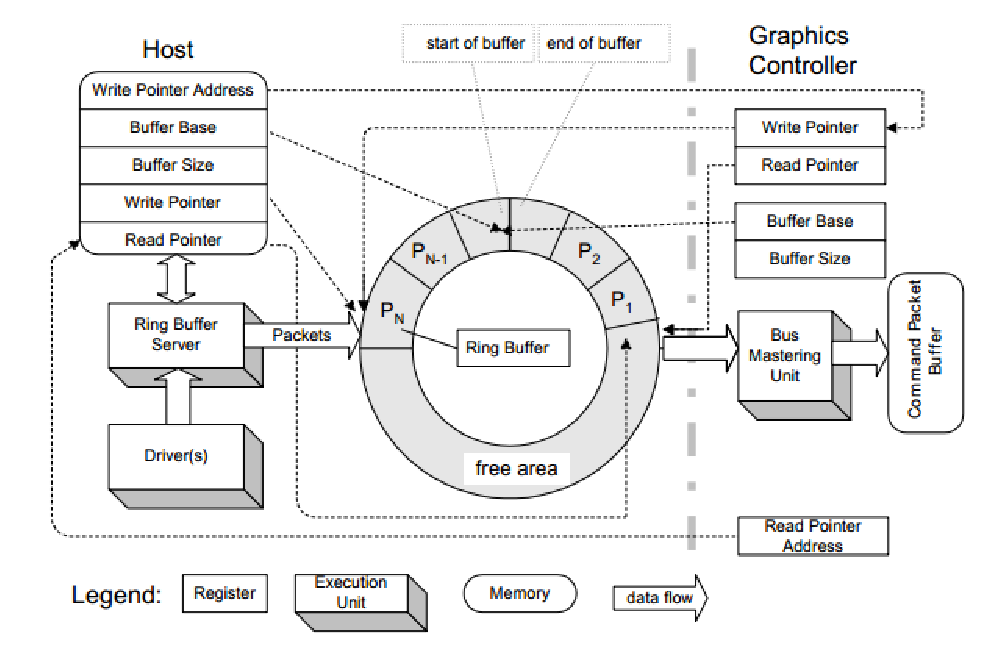
\includegraphics[width=16cm,height=12cm]{figures/chap03/CommandBuffer}
  \caption{Radeon R600系列显卡命令处理机制}
  \label{fig:CommandBuffer}
\end{figure}

如图\ref{fig:CommandBuffer},左边的Host(CPU)和右边的GPU各自记录了命令环的起始地址,并各自保存了一份读写指针,CPU写之前首先查询读指针,确认有空闲空间之后写入内容并更新写指针,GPU读取了命令之后更新读指针。CPU和GPU都要共同维护和管理环形缓冲区的状态:基地址、长度、写指针和读指针。为了使Ring Buffer能够正常工作,CPU和GPU必须维护这种状态的一致性。Ring Buffer基地址和大小是在系统第一次启动时已经初始化好的,之后一般也不会改变。当操作Ring Buffer时, 读指针和写指针的修改非常频繁。为了维护环形缓冲区的状态一致性,当写操作者(CPU)更新写指针时,它必须将写指针告诉GPU。同样的,当读操作者(GPU)更新读指针时,它必须将读指针告知CPU。无论是CPU还是GPU都是从低地址开始进行填写或抽取操作的,一旦到了环形缓冲区的结束处,又从环形缓冲区起始处继续\cite{Radeon-Manual}。  

上面提到的Radeon显卡命令是以命令包的形式出现的,如今Radeon系列显卡有4中命令包,分别是0型、1型、2型和3型命令包,命令包由两部分组成,第一部分是命令包头,第二部分是命令包主体,命令包头为请求GPU执行的具体操作,命令主体为执行该操作需要的数据。

下面分别介绍一下这四种命令包:

\begin{itemize}

\item{\textbf{0型命令包}} \\
0型命令包用于写连续N个寄存器。包主体部分是依次往这些寄存器写的值。包头各个部分的意义为:
\vspace{6pt}
\begin{center} \tablecaption{0型命令包 \label{tab:0-command}} 
\tablefirsthead{
\rowcolor[gray]{0.8}
\multicolumn{1}{l}{\textbf{位}} &
\multicolumn{1}{l}{\textbf{域名称}} &
\multicolumn{1}{c}{\textbf{描述}} \\ }
\tablehead{\multicolumn{3}{c}{
\small 表 \ref{tab:0-command} (续) } \\
\rowcolor[gray]{0.8}
\multicolumn{1}{l}{\textbf{位}} &
\multicolumn{1}{l}{\textbf{域名称}} &
\multicolumn{1}{c}{\textbf{描述}} \\ }
\tabletail{\bottomrule
\multicolumn{3}{c}{\small 接下页} \\}
\tablelasttail{\bottomrule}

\begin{supertabular}{p{2.cm}p{3.cm}m{10.cm}}
	12:0 & BASE\underline{ }INDEX & 要写的连续寄存器的第一个寄存器地址,最大地址0x7FFF \\
	14:13 & 保留位 & \\
	15 & ONE\underline{ }REG\underline{ }WR &  \\ 
	& & \tabitem 0表示将包主体的数据依次写入寄存器中 \\
	& & \tabitem 1表示所有数据写入同一个寄存器 \\
	29:16 & COUNT & 要写的寄存器数目N-1 \\
	31:30 & TYPE & 包类型,0型命令包类型名为0 \\
\end{supertabular}
\end{center}
\vspace{6pt}


\item{\textbf{1型命令包}} \\
1型命令包用于写两个的寄存器,1型命令包包头定义如下:
\vspace{6pt}
\begin{center} \tablecaption{1型命令包 \label{tab:1-command}} 
\tablefirsthead{
\rowcolor[gray]{0.8}
\multicolumn{1}{l}{\textbf{位}} &
\multicolumn{1}{l}{\textbf{域名称}} &
\multicolumn{1}{c}{\textbf{描述}} \\ }
\tablehead{\multicolumn{3}{c}{
\small 表 \ref{tab:1-command} (续) } \\
\rowcolor[gray]{0.8}
\multicolumn{1}{l}{\textbf{位}} &
\multicolumn{1}{l}{\textbf{域名称}} &
\multicolumn{1}{c}{\textbf{描述}} \\ }
\tabletail{\bottomrule
\multicolumn{3}{c}{\small 接下页} \\}
\tablelasttail{\bottomrule}

\begin{supertabular}{p{2.cm}p{3.cm}m{10.cm}}
	10:0 & REG\underline{ }INDEX1 & 第一个寄存器的地址 \\
	22:11 & REG\underline{ }INDEX2 & 第二个寄存器的地址 \\
	29:22 & RESERVED & 保留位 \\
	31:30 & TYPE & 1型命令包的类型为0x1 \\
\end{supertabular}
\end{center}
\vspace{6pt}

\item{\textbf{2型命令包}} \\
2型命令包是一个空命令包,用于填充对齐命令。2型命令包没有包主体,其包头最高两位为0x2,其它位无意义。

\item{\textbf{3型命令包}} \\
3型命令包是最功能最丰富的包,图形的主要功能都是通过这类包实现的。3型命令包主体内容由包头的IT\underline{ }OPCODE决定。3型命令是主要的命令包,涵盖了寄存器设置/绘图命令/同步等主要操作。3型命令包包头定义如下:
\vspace{6pt}
\begin{center} \tablecaption{3型命令包 \label{tab:3-command}} 
\tablefirsthead{
\rowcolor[gray]{0.8}
\multicolumn{1}{l}{\textbf{位}} &
\multicolumn{1}{l}{\textbf{域名称}} &
\multicolumn{1}{c}{\textbf{描述}} \\ }
\tablehead{\multicolumn{3}{c}{
\small 表 \ref{tab:3-command} (续) } \\
\rowcolor[gray]{0.8}
\multicolumn{1}{l}{\textbf{位}} &
\multicolumn{1}{l}{\textbf{域名称}} &
\multicolumn{1}{c}{\textbf{描述}} \\ }
\tabletail{\bottomrule
\multicolumn{3}{c}{\small 接下页} \\}
\tablelasttail{\bottomrule}

\begin{supertabular}{p{2.cm}p{3.cm}m{10.cm}}
	7:0 & reserved & 保留位 \\
	15:8 & IT\underline{ }OPCODE & 操作码 \\
	29:16 & COUNT & 包主题DWORDS数目-1 \\
	31:30 & TYPE & 3型包类型为0x3 \\
\end{supertabular}
\end{center}
\vspace{6pt}
\end{itemize}

\subsubsection{Mesa3D显示列表绘制模式实现原理}
\label{sec:display-list}

显示列表绘制模式即glGenList/glNewList/glEndList/glCallList,它可以提高性能,因为它存储OPENGL的函数,供以后使用,如果需要多次重绘同一个几何图形,或者如果一次需要多次调用的用于更改状态的函数,把这些函数存储在显示列表中,此时将显示列表中的矩阵结果集保存,后续使用不需要重复计算以提高性能。显示列表更像是命令缓存器,而不是动态数据库,也就是说当显示列表创建后,就无法修改。同时显示列表的创建也存在一定的系统开销,因此一个小的显示列表未必会提升性能。

我们以下面所示的svPerfGL测试集里面的显示列表模式为例,来看一下Mesa3D图形库是如何实现显示列表的绘制模式的。

\begin{lstlisting}
 // Create Display List
 glNewList(trianglesListIndx, GL_COMPILE);
 glDrawArrays(GL_TRIANGLES, 0, tNumVerts);
 glEndList(); 

 // Call Display List
 glCallList(trianglesListIndx);
\end{lstlisting}


当执行glNewList时,Mesa3D图形库会执行alloc\underline{ }vertex\underline{ }store函数预分配大小为VBO\underline{ }SAVE\underline{ }BUFFER\underline{ }SIZE*sizeof(GLfloat)的空白VRAM空间,这个空间我们姑且称之为buffer0。在显示列表机制下,保存模式的glDrawArrays只会执行一次,目的是将所有的顶点属性(位置、法线和颜色等)写入buffer0。VBO\underline{ }SAVE\underline{ }BUFFER\underline{ }SIZE的初值是8*1024,只能存放8*1024/3=2730个顶点属性,而glDrawArrays可能需要写入更多的顶点属性,因此buffer0是远远不够存放这些顶点属性的。当buffer0溢出后,显示列表会继续分配大小为VBO\underline{ }SAVE\underline{ }BUFFER\underline{ }SIZE * sizeof(GLfloat)的buffer1,buffer2,buffer3...直到所有顶点属性都写入VRAM。可见,当glDrawArray执行完时,所有的顶点属性已经存入VRAM,但是分散在很多个小buffer中。

接着通过执行glCallList来调用已保存好顶点属性的显示列表,glCallList将执行vbo\underline{ }save\underline{ }playback\underline{ }vertex\underline{ }list函数来实现渲染,该函数调用r600\underline{ }draw\underline{ }vbo向GPU发如下命令:

\begin{lstlisting}
cs->buf[cs->cdw++] = PKT3(PKT3_DRAW_INDEX_AUTO, 1, 
                          rctx->predicate_drawing);
cs->buf[cs->cdw++] = info.count;
cs->buf[cs->cdw++] = V_0287F0_DI_SRC_SEL_AUTO_INDEX 
                     | (info.count_from_stream_output? 
                        S_0287F0_USE_OPAQUE(1) : 0);
\end{lstlisting}

这些命令通过Command Stream机制被GPU读取并执行,从而启动pipeline进行3D渲染。

\begin{figure}[H] 
  \centering
  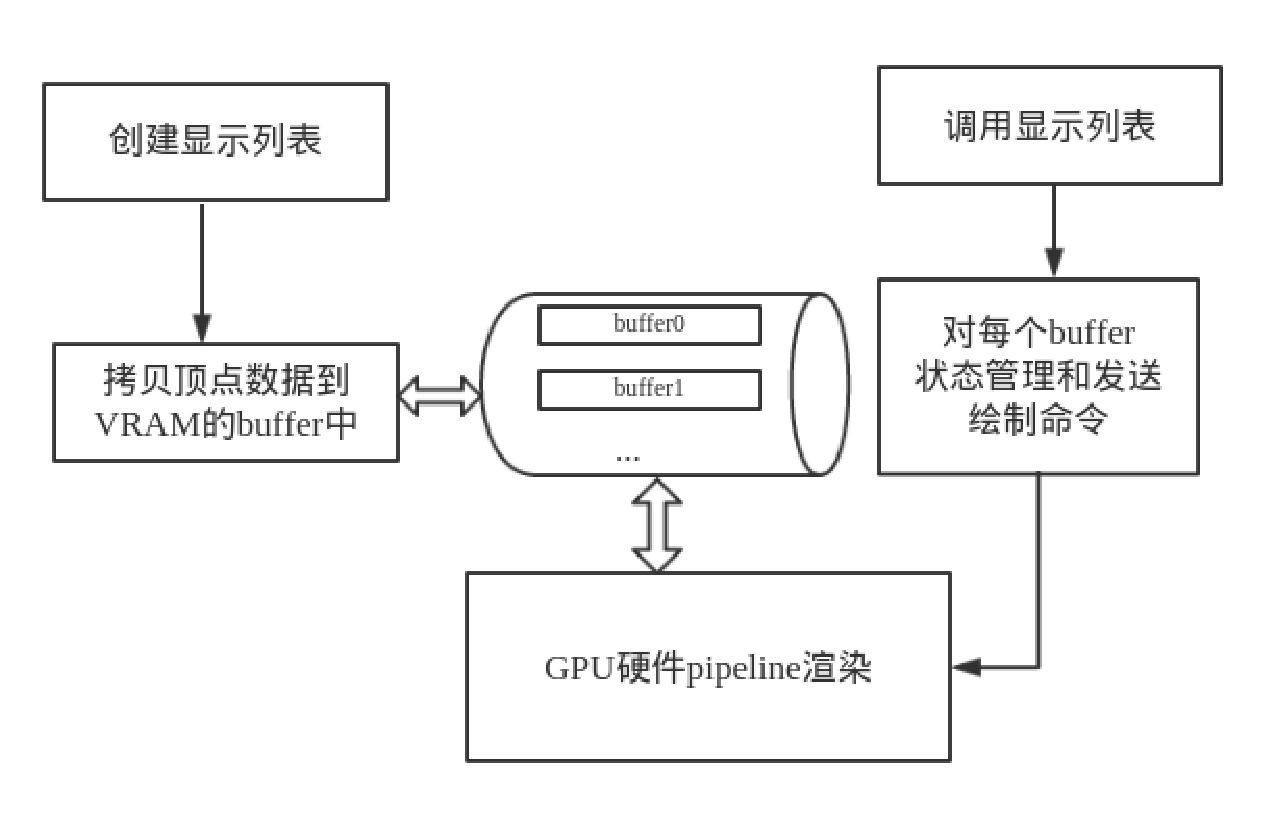
\includegraphics[width=12cm,height=10cm]{figures/chap03/display-list-flow}
  \caption{Mesa3D图形库显示列表实现机制}
  \label{fig:display-list-flow}
\end{figure}

由于显示列表是一次创建多次调用,所以如图\ref{fig:display-list-flow}所示,每次在调用显示列表时候都会做对每个buffer进行状态管理和发送绘制命令到GPU。GPU在执行完3D渲染之后将结果放入framebuffer中然后通过显示设备显示出来。

\subsection{CPU与GPU负载分析}

我们在前面就介绍过Radeon R600系列GPU的工作模型就是CPU端将数据和命令写入Command Buffer中,然后GPU读取Command Buffer中的命令并执行(图\ref{fig:CommandBuffer})。所以从这个模型我们可以看到这里存在着CPU/GPU的负载平衡问题:如果CPU端执行效率比GPU端执行效率更快,那么会导致Command Buffer满载,这样CPU就不得不需要同步操作停下来等待GPU处理完命令以得到Command Buffer里面一些空闲的位置继续写入命令;同样,如果GPU端执行的效率更高,这样每当CPU写完命令之后GPU就可以很快的执行完毕,这样Command Buffer常常会处于空闲状态,GPU就不得不空闲下来等待CPU的处理结果。不论是哪一种情况都属于CPU与GPU的负载不平衡,这样都会造成性能的瓶颈。

从前面的分析里面我们可以知道显示列表模式的CPU和GPU的协同工作模型就是:CPU数据准备与状态管理、GPU处理数据、CPU数据准备与状态管理、GPU处理数据、反复直至数据全部处理完毕。那么现在我们就从CPU与GPU的负载平衡的关系上来看我们将上面提到的svPerfGL里面的显示列表模式测试项的情况。这里测试每帧100万个三角形的绘制时候CPU和GPU的负载状况。测试结果如下图\ref{fig:cpu-load-dsp}和图\ref{fig:gpu-load-dsp}

\begin{figure}[H]
  \begin{minipage}[t]{0.5\linewidth} 
  \centering
  \includegraphics[width=8cm,height=6cm]{figures/gnuplot/dsp/cpu-load}
  \caption{显示列表测试项CPU负载}
  \label{fig:cpu-load-dsp}
  \end{minipage}
  \begin{minipage}[t]{0.5\linewidth} 
  \centering
  \includegraphics[width=8cm,height=6cm]{figures/gnuplot/dsp/gpu-load}
  \caption{显示列表测试项GPU负载}
  \label{fig:gpu-load-dsp}
  \end{minipage}
\end{figure}

从上面的图中我们可以看到CPU的负载情况明显比GPU要大很多,这里的原因也很好解释: 如前面章节\ref{sec:display-list}研究的那样,对每一次的buffer,Mesa3D需要都先在CPU端数据准备和状态管理,然后提交给GPU处理。这里当我们绘制大量的顶点时候,例如glDrawArray函数里面写入100万个三角形,那么每个三角形需要有3个顶点*3钟顶点属性(位置、法线和颜色),所以一种有1000000*3*3即9000000个顶点属性,根据前面分析的默认的buffer大小是8*1024*4字节,那么总共需要的buffer数目就是9000000*3*4/(8*1024*4)即3296个。由于对这3296个buffer每一个都需要CPU进行进行数据准备和状态管理等大量操作,这对性能较为优越的X86不是问题,却能极大的消耗龙芯3A的CPU。这样也就造成了CPU负载过大,而GPU负载较小的结果。


\subsection{CPU与GPU负载平衡优化}

由前一节分析我们可以看到CPU负载过大导致了CPU与GPU负载不平衡问题,究其原因就是CPU端需要处理的buffer数目过多,于是本文提出了一种通过调整显示列表缓存buffer大小的方法来优化显示列表的CPU与GPU负载不平衡问题。

如前面章节\ref{sec:display-list}所分析的那样,显示列表由于数据都已经上传保存到VRAM中的buffer里面,所以每次调用显示列表时候并不需要再次上传数据,而只是对每个buffer进行数据准备和状态管理即可,这些工作与buffer所装载的数据大小并没有关系,于是我们可以将buffer的大小调整到一个合适的数值,然后使得CPU的负载降低,GPU的负载增加以提高整体性能。

为了寻找显示列表缓存buffer的合适大小,我们通过测试svPerfGL显示列表程序在60秒内绘制每帧100万个三角形的绘制性能来确定这一合适值。相关测试结果如下表\ref{tab:buffer-performance}:

\begin{center} \tablecaption{svPerfGL显示列表测试项不同buffer大小下绘制性能 \label{tab:buffer-performance}} 
\tablefirsthead{
\rowcolor[gray]{0.8}
\multicolumn{1}{c}{\textbf{buffer大小}} &
\multicolumn{1}{c}{\textbf{帧数}} &
\multicolumn{1}{c}{\textbf{渲染效率(frame/s)}} \\ }
\tablehead{\multicolumn{3}{c}{
\small 表 \ref{tab:0-command} (续) } \\
\rowcolor[gray]{0.8}
\multicolumn{1}{c}{\textbf{buffer大小}} &
\multicolumn{1}{c}{\textbf{帧数}} &
\multicolumn{1}{c}{\textbf{渲染效率(frame/s)}} \\ }
\tabletail{\bottomrule
\multicolumn{3}{c}{\small 接下页} \\}
\tablelasttail{\bottomrule}

%./svPerfGL -i ../../trisNormsColors-512.nc -w 1280 -h 1024 -2 -r -t 60 -s 3000000
\begin{supertabular}{p{6.cm}p{3.cm}m{6.cm}}
	32K& 169& 2.81\\
	64K& 250& 4.16\\
	128K& 241& 4.01\\
	256K& 242& 4.03\\
	512K& 266& 4.42\\
	1024K& 268& 4.46\\
	2048K& 269& 4.47\\
	4096K& 209& 3.47\\
\end{supertabular}
\end{center}

根据测试结果,我们可以发现将buffer的大小设定为2048KB能够取得较好的性能。此时再次测量CPU和GPU的负载状况如图\ref{fig:cpu-load-dsp-opt}和图\ref{fig:gpu-load-dsp-opt}:

\begin{figure}[H] 
  \begin{minipage}[t]{0.5\linewidth} 
  \centering
  \includegraphics[width=8cm,height=6cm]{figures/gnuplot/dsp/cpu-load-opt}
  \caption{显示列表测试项优化后CPU负载}
  \label{fig:cpu-load-dsp-opt}
  \end{minipage}
  \begin{minipage}[t]{0.5\linewidth} 
  \centering
  \includegraphics[width=8cm,height=6cm]{figures/gnuplot/dsp/gpu-load-opt}
  \caption{显示列表测试项优化后GPU负载}
  \label{fig:gpu-load-dsp-opt}
  \end{minipage}
\end{figure}

可以看到此时GPU刚好达到了满载,CPU负载较轻,因为龙芯平台CPU处理能力较GPU的处理能力稍弱,所以这样的负载关系比较符合当前硬件特点,所以能够取得较好的性能提升。

当然buffer大小调整这种优化方法也有一定的缺点,我们将buffer的大小调大的时候会增加VRAM的管理粒度,在小数据规模时候可能会造成VRAM的浪费,特别是在某些显卡显存比较紧俏的机器环境下可能会消耗掉所有的VRAM空间,造成VRAM空间不够程序无法执行的问题。所以这个优化方法可以作为可配置的优化手段,在实际工程应用中可以根据具体硬件情况进行选择。


\section{Mesa3D的内存到显存的数据传输的优化}

\subsection{研究背景}

\subsubsection{Mesa3D顶点数组绘制模式实现原理}
从前面的立即模式实现原理我们可以看到顶点数据是一个个的搬运到VRAM上的buffer上的,当我们绘制拥有大量数据的图形时候,这样一点点的搬运就显得非常的缓慢了,当然我们可以尝试使用显示列表来对这些数据进行预编译,需要遍历这些顶点数据然后把数据传给GPU的显存。但是这些数据不一定是静态的,有可能在我们每次渲染的时候,我们需要对这些数据进行更改。这个时候就不适合使用显示列表了。

为了很好的解决这个问题。我们可以使用顶点数组,我们可以随时进行预编译或修改几何图形,然后一次性传输这些数据。顶点数组的绘制模式相对于立即模式极大的提高了绘制效率。使用顶点数组有3个基本的步骤:

\begin{itemize}
\item{} 激活(启用)最多可达8个数组,每个数组用于存储不同类型的数据: 顶点坐标,表面法线,颜色等等。
\item{} 把数据放入数组中。这些数组是通过它们的内存位置的地址(即指针)进行访问。
\item{} 用这些数据绘制几何图形。OpenGL通过指针从所有激活的数组中获取数据。
\end{itemize}

我们还是以svPerfGL的顶点数组模式测试项为研究对象来分析Mesa3D顶点数组的实现原理:

\begin{lstlisting}
glEnableClientState(GL_VERTEX_ARRAY);
glVertexPointer(3, GL_FLOAT, sizeof(float)*3, (const GLvoid *)tVerts);
glEnableClientState(GL_NORMAL_ARRAY);
glNormalPointer(GL_FLOAT, sizeof(float)*3, (const GLvoid *)tNorms);
glEnableClientState(GL_COLOR_ARRAY);
glColorPointer(3, GL_FLOAT, sizeof(float)*3, (const GLvoid *)tColors);

glDrawArrays(GL_TRIANGLES, 0, tNumVerts);
\end{lstlisting}

这里在介绍Mesa3D顶点数组实现原理之前先介绍一个重要的数据结构:
\begin{lstlisting}
struct pipe_vertex_buffer{
   ...
   struct pipe_resource *buffer; 
   const void *user_buffer;
};

struct pipe_vertex_buffer vertex_buffer[PIPE_MAX_ATTRIBS];
\end{lstlisting}
这里vertex\underline{ }buffer数组就是存放着各个属性数据数组的指针,当我们使用传统的立即模式时候,这些指针就指向着前面一节说到的VRAM上的buffer(struct pipe\underline{ }resource *buffer),而在我们使用顶点数组模式时候,这些指针就指向着我们用户准备的顶点数据数组(const void *user\underline{ }buffer)。所以在顶点数组模式下,在glVertexPointer()这类函数执行时候,Mesa3D会把用户指定的数组指针添加到对应vertex\underline{ }buffer[]数组里面的user\underline{ }buffer中。接着我们调用glDrawArrays()之类的函数进行顶点数组模式绘制时候,Mesa3D会执行u\underline{ }vbuf\underline{ }upload\underline{ }buffers函数将用户定义的顶点数组数据通过memcpy()函数从内存拷贝到显存中,然后像之前的立即模式一样向GPU发送绘制命令执行硬件渲染。

\begin{figure}[H] 
  \centering
  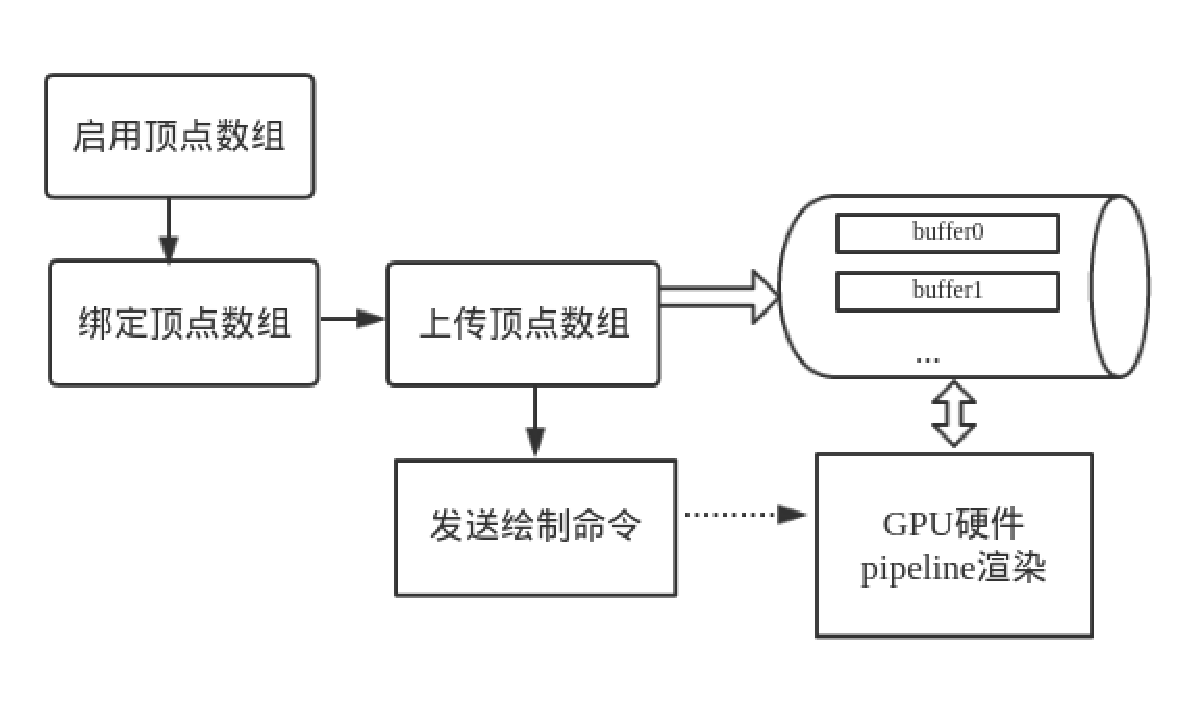
\includegraphics[width=12cm,height=8cm]{figures/chap03/vbo-flow}
  \caption{Mesa3D图形库顶点数组模式实现机制}
  \label{fig:vbo-flow}
\end{figure}

顶点数组模式绘制的简要流程如图\ref{fig:vbo-flow}所示,这里需要说明的是顶点数组模式下在VRAM上创建的buffer大小是依据用户定义的数组大小而定的,并不像立即模式那样有着固定的大小,一旦填满就开始部分绘制,顶点数组模式是把所有数据都传递到显存之后再一次性的GPU绘制,由于是一次性memecpy的大数据传输,所以传输效率上要比传统的立即模式快的多,这也是后来OpenGL标准中增加顶点数组模式的原因。

\subsubsection{内存与显存数据传输优化的意义}

在一般的GPU硬件加速的程序应用场景中,内存到显存的数据传输是不可避免的,Chris Gregg等人在论文Where is the Data? Why You Cannot Debate CPU vs. GPU Performance Without the Answer\cite{Where-is-the-Data}里面以十多项常见的GPU应用程序为benchmark,通过测试和分析不同数据规模下的benchmark运行效率发现内存与显存之间的数据传输几乎对所有的GPU应用程序运行性能都有着十分重要的影响。特别是在大数据输入集下,内存与显存传输的时间开销最高可以达到GPU计算时间开销的50多倍。由此我们可以得到结论:内存与显存的数据传输是影响GPU应用程序性能的重要的因素。


\subsubsection{CPU与GPU的访存机制}

我们首先介绍以下GPU的访存机制。GPU使用的内存分为两个部分,一部分是显卡自带的显存称为VRAM(Vedio RAM),另一部分是系统主存(即CPU端内存)也称为GTT内存。为了实现GPU同时使用VRAM内存和GTT内存最简单的方法就是将这两片内存统一编址,VRAM是显卡自带的内存,它的地址一定是连续的,但是不连续的GTT内存如果要统一编址,那么一定需要通过建立页表映射关系,这个页表也就是GTT(graphics translation table, 地址转换表)。

和CPU的地址类似,GPU直接使用的地址被称为“GPU虚拟地址”,经过查页表转化之后的地址称为“GPU物理地址”,也就是GPU最终真实访问的地址,其中GPU的虚拟地址和物理地址转换过程如图\ref{fig:gpu-mmu}所示:对于属于GTT的虚拟地址,通过查找GPU页表找到真实的PCI地址,然后通过PCI地址访问系统主存;对于属于VRAM的虚拟地址则无须页表转换直接在VRAM内寻址。

\begin{figure}[H] 
  \centering
  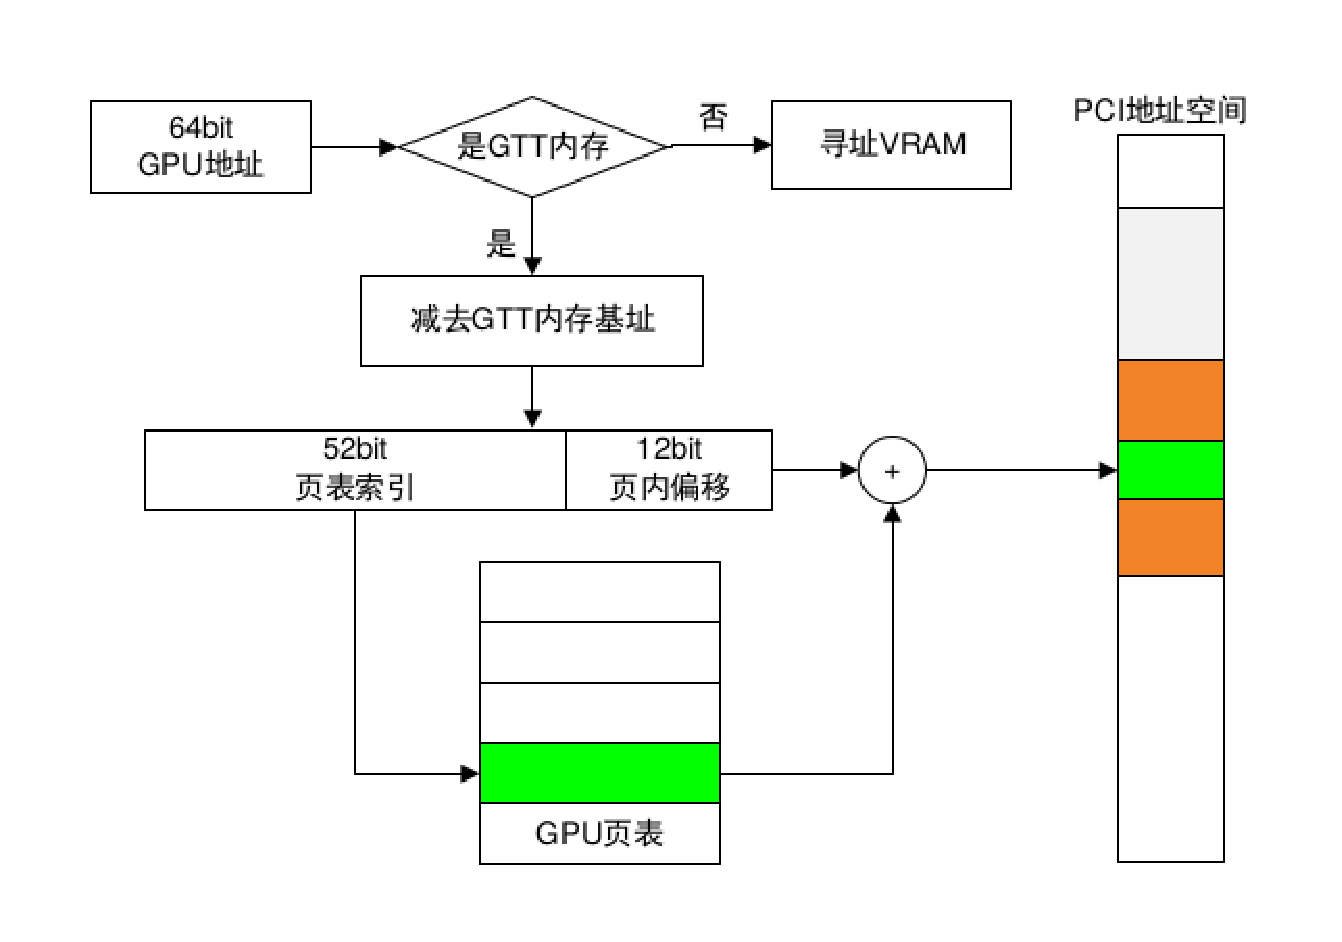
\includegraphics[width=12cm,height=8cm]{figures/chap03/gpu-mmu}
  \caption{GPU的内存访问机制}
  \label{fig:gpu-mmu}
\end{figure}

与此同时,CPU使用的内存就复杂的多了,CPU通过MMU单元将虚拟地址转化成实际的物理地址,这些物理地址有的是系统主存的地址,有些是外接设备的地址,其中就包括GPU的自带显存VRAM地址。通过下图\ref{fig:cpu-gpu-mm}可以看到,CPU和GPU均能自有访问系统内存和显卡内存VRAM。

\begin{figure}[H] 
  \centering
  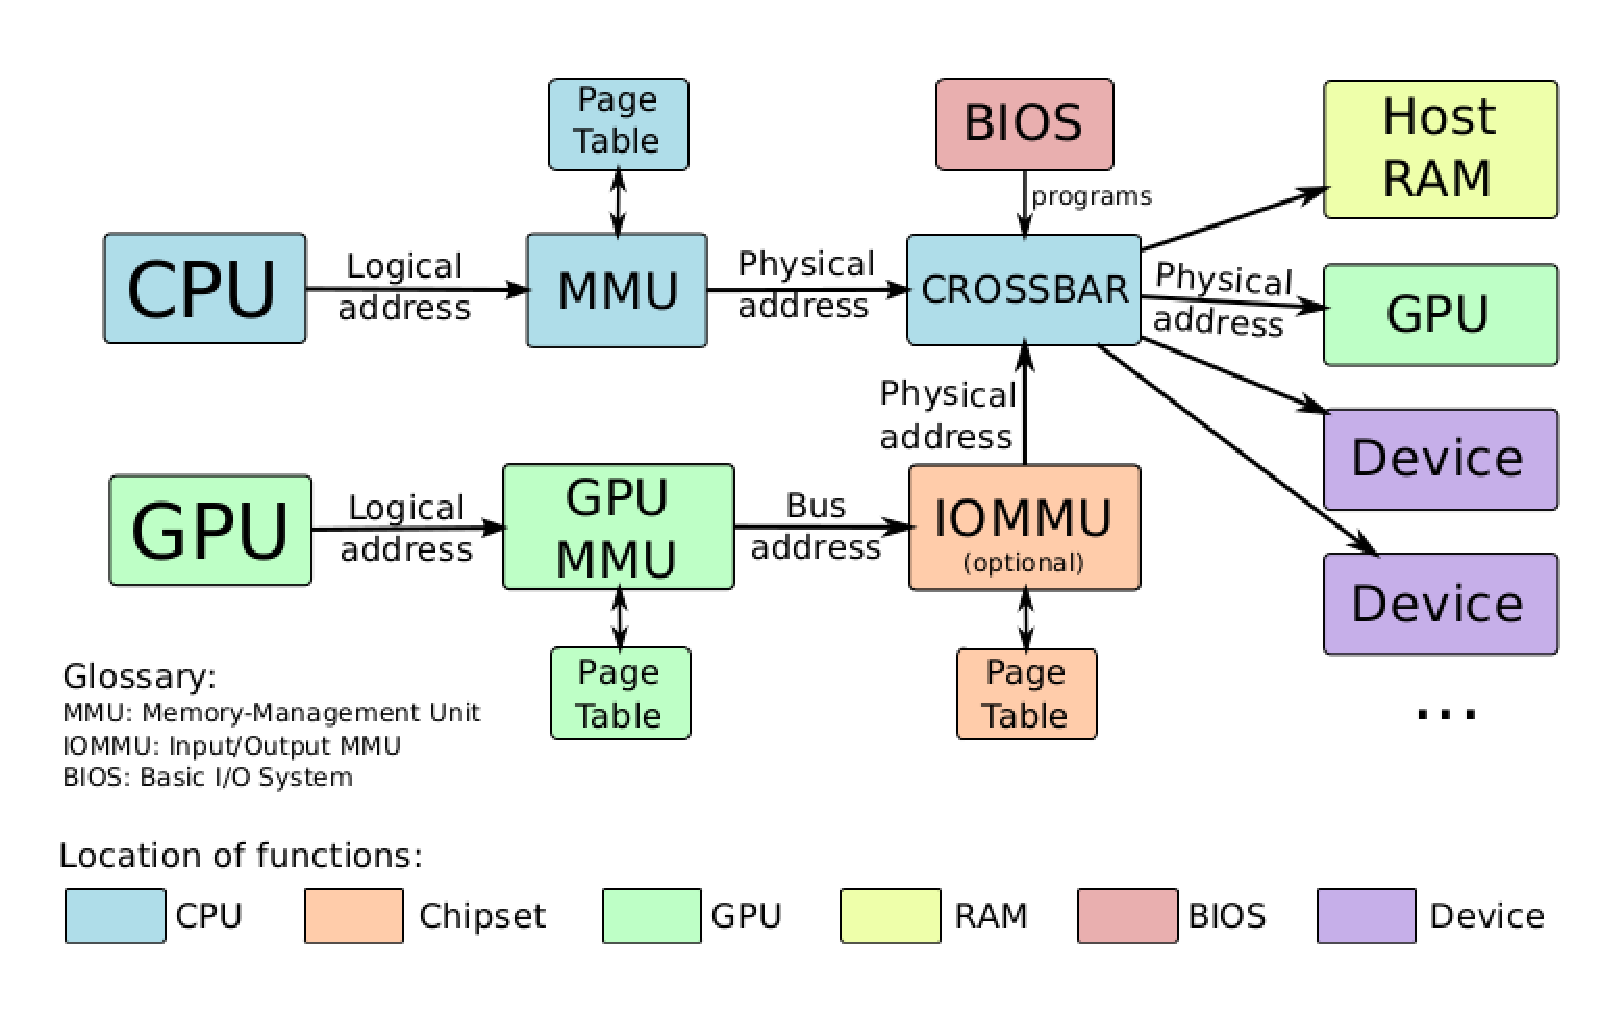
\includegraphics[width=12cm,height=8cm]{figures/chap03/cpu-gpu-mm}
  \caption{CPU与GPU内存请求回路}
  \label{fig:cpu-gpu-mm}
\end{figure}

\subsubsection{龙芯平台下内存与显存传输的性能分析}

从CPU的角度来说我们可以看到存在着两种内存传输: 系统内存到系统内存(cache)、系统内存到显存。这里本文以龙芯3A搭载Radeon R600显卡平台为例测试并研究这两种传输的性能。得到相关数据如下表\ref{tab:memcpy-performance}所示:

\begin{center} \tablecaption{龙芯3A访存性能分析 \label{tab:memcpy-performance}} 
\tablefirsthead{
\rowcolor[gray]{0.8}
\multicolumn{1}{c}{\textbf{数据量大小}} &
\multicolumn{1}{c}{\textbf{内存到内存}} &
\multicolumn{1}{c}{\textbf{内存到显存}} \\ }
\tablehead{\multicolumn{3}{c}{
\small 表 \ref{tab:memcpy-performance} (续) } \\
\rowcolor[gray]{0.8}
\multicolumn{1}{c}{\textbf{数据量大小}} &
\multicolumn{1}{c}{\textbf{内存到内存}} &
\multicolumn{1}{c}{\textbf{内存到显存}} \\ }
\tabletail{\bottomrule
\multicolumn{3}{c}{\small 接下页} \\}
\tablelasttail{\bottomrule}

%./svPerfGL -i ../../trisNormsColors-512.nc -w 1280 -h 1024 -2 -r -t 60 -s 3000000
\begin{supertabular}{p{5.cm}<{\centering}p{5.cm}<{\centering}m{6.cm}<{\centering}}
	4KB& 409MB/s& 12MB/s\\
	16KB& 564MB/s& 14MB/s\\
	64KB& 313MB/s& 14MB/s\\
	256KB& 268MB/s& 14MB/s\\
	1MB& 246MB/s& 14MB/s\\
	4MB& 210MB/s& 14MB/s\\
	16MB& 201MB/s& 14MB/s\\
	64MB& 185MB/s& 14MB/s\\
	256MB& 178MB/s& 14MB/s\\
\end{supertabular}
\end{center}

通过上表\ref{tab:memcpy-performance}我们可以发现龙芯3A平台上内存到显存拷贝效率较低,这里主要是因为内存到显存拷贝数据传输是通过PCI-E总线传输的,而龙芯平台上PCI-E带宽非常的小,所以导致这样直接传输的性能底下。

\subsection{Mesa3D图形库CPU与GPU访存行为分析}

在Mesa3D图形库的实现中,CPU端在初始化过程中会创建顶点对象缓存区,而这些顶点对象缓存区是创建在VRAM之上的,然后通过内存映射的方式映射成CPU端虚拟地址进行访问。在上层程序需要使用Mesa3D进行图形绘制时候,Mesa3D会将绘制相关的顶点数据拷贝到顶点对象缓存区中,即发生了CPU端内存到显存的拷贝,整个过程是同步实现的,即需要占用CPU的指令周期。当GPU接受到绘制命令和相关顶点数据准备好时候,GPU就开始内部的硬件图形加速渲染管线进行图形渲染,并将渲染结果放置到显存的framebuffer中以待显示。以svPerfGL程序顶点数组测试项为例,假如我们需要每帧绘制100万个三角形,那么就会发生三次顶点数据拷贝,分别是顶点位置、顶点颜色和顶点法向量信息,每次拷贝数据量是100万*3*3*4B即36MB数据的大小。

通过上表\ref{tab:memcpy-performance}我们可以看到从内存拷贝到显存这么多数据是非常缓慢的,并且我们通过perf工具测试出整个顶点数组模式测试项的执行时间中百分之九十的时间都花在这个拷贝数据之上,所以成为了程序的性能瓶颈。

\subsection{Mesa3D图形库CPU与GPU访存优化}

针对Mesa3D图形库实际的访存特点,本文从访存策略与拷贝效率这两个方面提出了相应的优化方案。

\subsubsection{CPU与GPU访存策略的优化}
从前面的介绍我们知道,由于CPU端内存到显存的数据拷贝效率低下,导致占用了大量的CPU执行周期,使得CPU执行时间占比过大,而GPU相对执行时间过少。为了改变这一状况,如下图\ref{fig:vbo-gtt}我们可以把顶点数据缓冲区创建在系统内存之上,CPU只需简单的系统内存内部搬运数据,而GPU则通过GTT的方式访问顶点数据缓冲区然后进行图形硬件渲染。

\begin{figure}[H] 
  \centering
  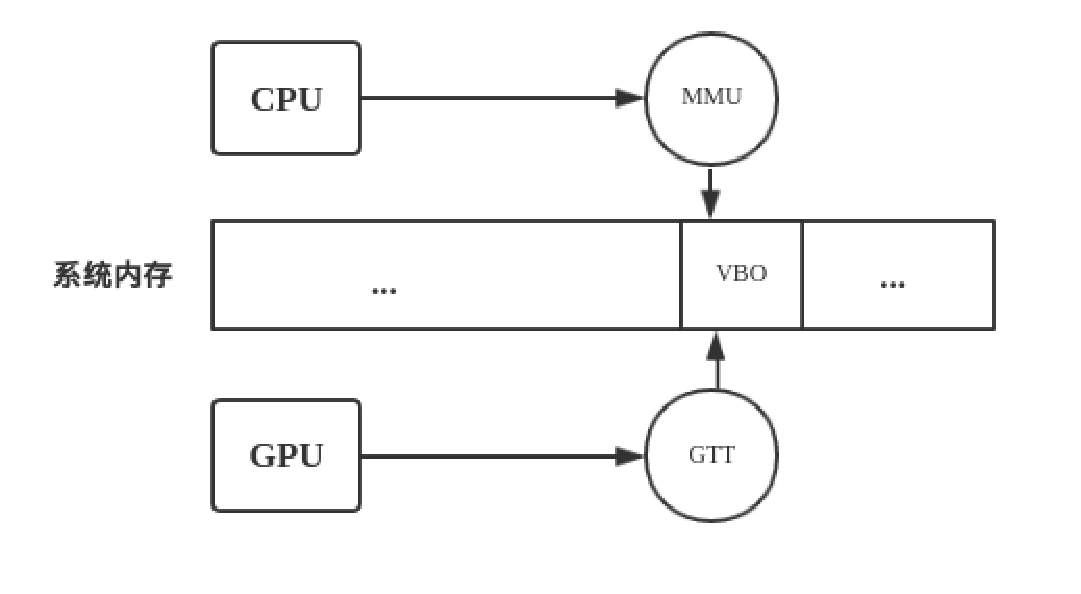
\includegraphics[width=10cm,height=6cm]{figures/chap03/vbo-gtt}
  \caption{Mesa3D图形库CPU与GPU改进后访存策略}
  \label{fig:vbo-gtt}
\end{figure}

虽然这样之后,GPU渲染时候的数据访问效率会降低,但是由于本身GPU工作负担小于CPU,而且因为龙芯平台CPU执行效率相对GPU较弱,所以整个CPU和GPU的并行程度提高了,缩短了整个的执行时间。

\subsubsection{CPU拷贝效率的优化}

在前一节的改进访存策略之后,我们可以通过提高拷贝效率来改进CPU的数据传输性能。由于CPU端向GTT的数据拷贝大多都是单精度浮点数据的拷贝,所以我们可以通过龙芯平台特有的宽位访存指令来提高拷贝效率。

\textbf{龙芯扩展宽位访存指令}: 龙芯平台为了自身发展的需求,通过龙芯指令系统融合技术\cite{loongson-merge},专门开发了一些宽位访存指令,诸如本文使用到的128bit浮点访存指令GSLQ和GSSQ可以实现128bit的浮点数据存取。

由于我们的宽位访存指令GSLQ和GSSQ必须要按照要求先进行128位对齐后使用,所以我们在优化CPU的单精度浮点数据拷贝时候,则必须要考虑到拷贝源地址和目的地址的对齐情况,为了更简明的说明这个问题,我们可以通过下图\ref{fig:memcpy}来看宽位访存指令实现拷贝效率优化的整个过程。

\begin{figure}[H] 
  \centering
  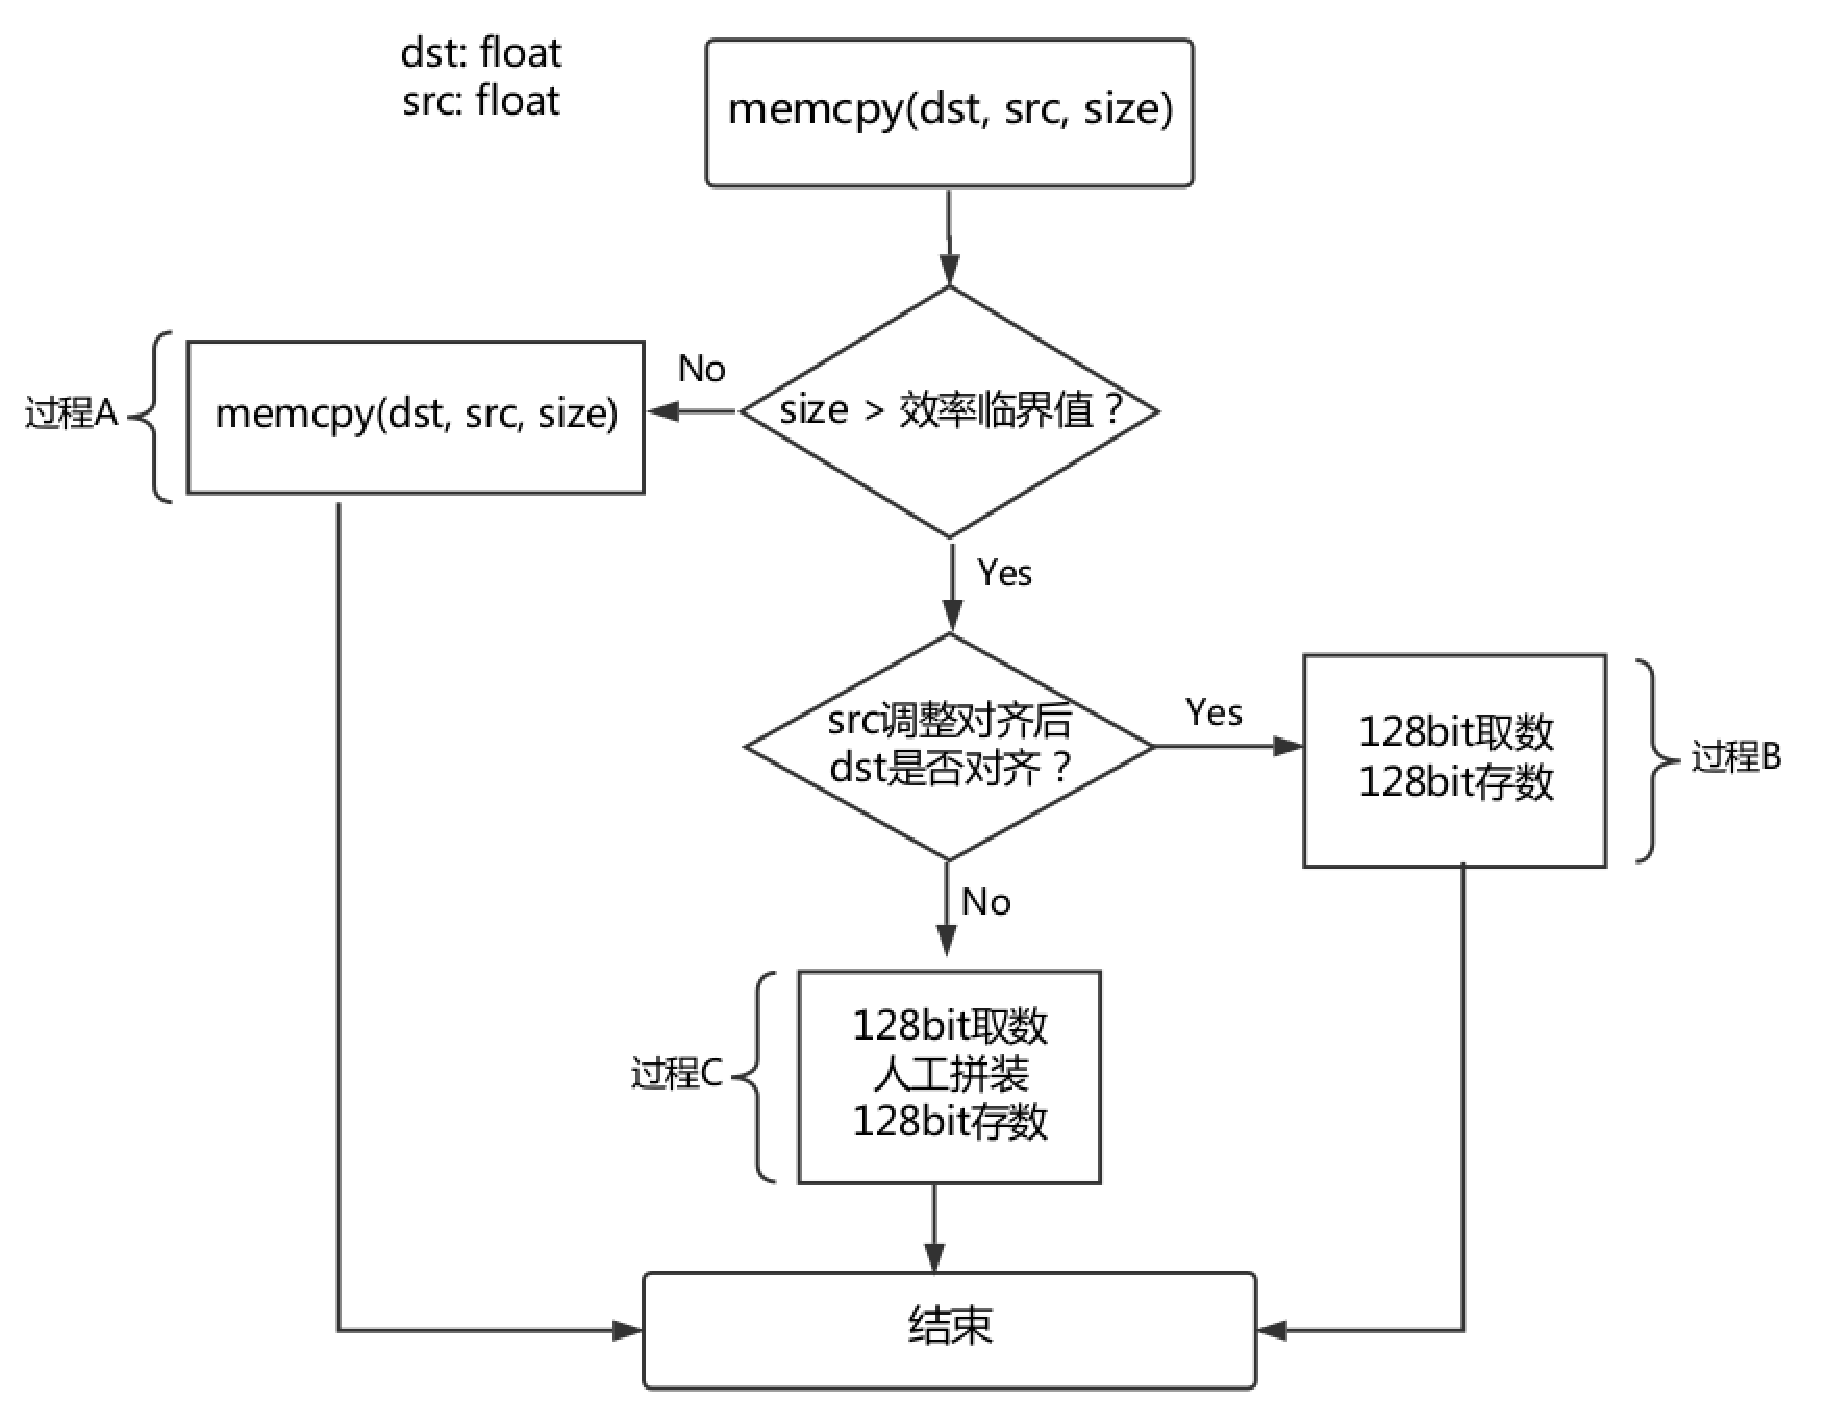
\includegraphics[width=16cm,height=9cm]{figures/chap03/memcpy}
  \caption{宽位访存指令实现拷贝效率优化}
  \label{fig:memcpy}
\end{figure}

这里介绍一下流程图\ref{fig:memcpy}里面的过程A、过程B和过程C的具体工作:

\begin{itemize}

\item{\textbf{过程A}}: 直接调用glibc系统库的memcpy函数。
\item{\textbf{过程B}}: \\
因为这种情况下源地址src和目的地址dst都是128bit对齐的,所以只需要直接的使用宽位访存指令取数和存数即可。相关实现伪代码如下:
\vspace{6pt}
\begin{breakablealgorithm}
	\caption{过程B算法}
	\begin{algorithmic}[1] %每行显示行号
		\Require $dst$目的地址,$src$源地址, $size$大小
		%\Ensure 
		\Function {memcpy}{$dst, src, size$}
			\State $gpr0 \gets src$
			\State $gpr1 \gets dst$
			\State $off \gets 0$
			\While {$off + 16 < size$}
				\State $gslq\, gpr2,\, gpr1,\, off(gpr0)$
				\State $gssq\, gpr2,\, gpr1,\, off(gpr1)$
				\State $off \gets off + 16$
			\EndWhile
		\EndFunction
	\end{algorithmic}
\end{breakablealgorithm}
\vspace{6pt}

\item{\textbf{过程C}}: \\
由于在源地址src对齐后,目的地址dst不是128bit对齐的,所以这里目的地址dst与128bit对齐地址的差可能会是32bit、64bit和96bit这三种,然后无论哪一种都需要我们进行人工的暂存和拼接组装。实现伪代码如下:
\vspace{6pt}
\begin{breakablealgorithm}
	\caption{过程C算法}
	\begin{algorithmic}[1] %每行显示行号
		\Require $dst$目的地址,$src$源地址, $size$大小
		%\Ensure 
		\Function {memcpy}{$dst, src, size$}
			\State $array pre[0:3] \gets \{0.0f, 0.0f, 0.0f, 0.0f\}$
			\State $array cur[0:3] \gets \{0.0f, 0.0f, 0.0f, 0.0f\}$
			\State $offbit \gets (dst \% 16) * 8$
			\State $n \gets offbit/32 - 1$
			\State $pre[0:n] \gets src[0:n]$
			\State $off \gets 16$
			\State $gpr0 \gets src + off$
			\State $gpr1 \gets dst + off - offbit/8$
			\While {$off + 16 < size$}
				\State $gslq\, gpr2, gpr3, off(gpr0)$
				\State $cur[n+1:3]  \gets \{gpr2, gpr3\}\, low\, 128-offbit\, bit$
				\State $cur[0:n] \gets pre[0:n]$
				\State $pre[0:n] \gets \{gpr2, gpr3\}\, high\, offbit\, bit$
				\State ${gpr2, gpr3} \gets cur[0:3]$
				\State $gssq\, gpr2,\, gpr3,\, off(gpr1)$
				\State $off \gets off + 16$
			\EndWhile
		\EndFunction
	\end{algorithmic}
\end{breakablealgorithm}
\vspace{6pt}

\end{itemize}

这里以目的地址dst与128bit对齐地址偏移32bit为例来解释上述过程C算法。如下图\ref{fig:offset32}所示,我们需要将src开始的源数据搬运到dst开始的目的位置,此时src已经是128bit对齐,而dst与128bit对齐相差32bit,这时我们将s4位置的32bit数据暂存起来,接着采用宽位访存指令读取src下一个128bit数据,即\{s5,s6,s7,s8\},接着我们将s4,s5,s6,s7拼装起来成128bit采用宽位访存指令存储到dst的下一个128bit对齐位置,即{d4,d5,d6,d7}。以此规律循环处理即可完成非对齐情况下的数据拷贝。


\begin{figure}[H] 
  \centering
  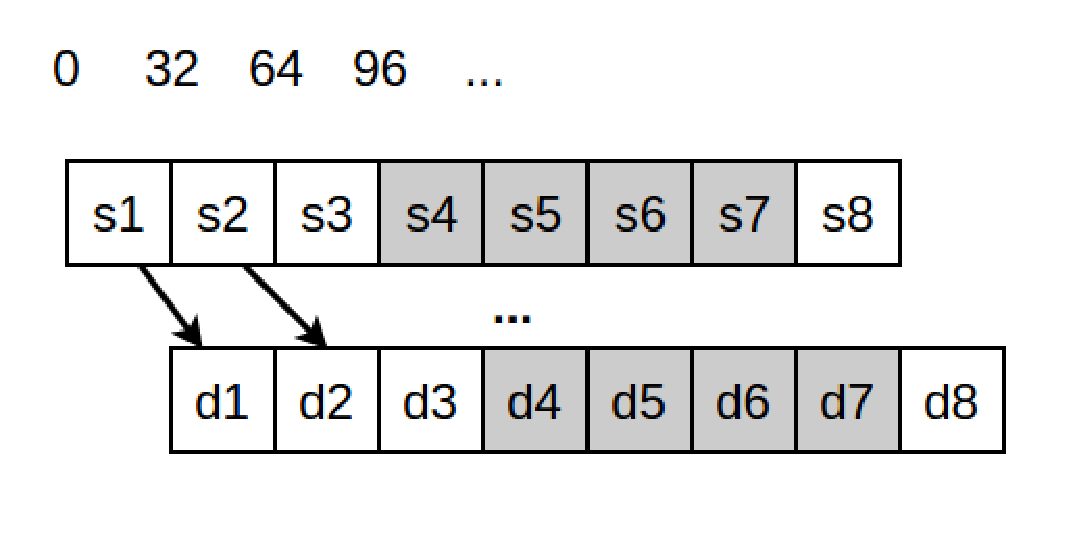
\includegraphics[width=10cm,height=6cm]{figures/chap03/offset32}
  \caption{32bit偏移下过程C算法举例}
  \label{fig:offset32}
\end{figure}

这里为了验证宽位访存指令的效果,进行了内存到内存的拷贝性能测试,测试结果如下:

\begin{center} \tablecaption{宽位访存指令优化效果测试 \label{tab:memcpy-performance-opt}} 
\tablefirsthead{
\rowcolor[gray]{0.8}
\multicolumn{1}{c}{\textbf{数据量大小}} &
\multicolumn{1}{c}{\textbf{优化前}} &
\multicolumn{1}{c}{\textbf{优化后}} \\ }
\tablehead{\multicolumn{3}{c}{
\small 表 \ref{tab:memcpy-performance-opt} (续) } \\
\rowcolor[gray]{0.8}
\multicolumn{1}{c}{\textbf{数据量大小}} &
\multicolumn{1}{c}{\textbf{优化前}} &
\multicolumn{1}{c}{\textbf{优化后}} \\ }
\tabletail{\bottomrule
\multicolumn{3}{c}{\small 接下页} \\}
\tablelasttail{\bottomrule}

%./svPerfGL -i ../../trisNormsColors-512.nc -w 1280 -h 1024 -2 -r -t 60 -s 3000000
\begin{supertabular}{p{6.cm}<{\centering}p{3.cm}<{\centering}m{6.cm}<{\centering}}
	4KB& 409MB/s& 819MB/s\\
	16KB& 564MB/s& 1260MB/s\\
	64KB& 313MB/s& 420MB/s\\
	256KB& 268MB/s& 399MB/s\\
	1MB& 246MB/s& 325MB/s\\
	4MB& 210MB/s& 227MB/s\\
	16MB& 201MB/s& MB/s\\
	64MB& 185MB/s& MB/s\\
	256MB& 178MB/s& 183MB/s\\
\end{supertabular}
\end{center}

\subsubsection{GPU拷贝效率的优化}

前面提到的CPU与GPU拷贝策略的优化是把数据放在GTT,然后让GPU来GTT访问数据,这样可能会加大GPU的负载,所以这里采用张凯的论文$<<$显存与内存间的数据传输通路优化$>>$\cite{gpu-cpu-data}里面提到采用GTT+DMA的这种非线性的优化方法,使用这种方法的原理就是GPU采用DMA的方式在不占用CPU的执行周期的情况下将GTT里面的内容快速的拷贝到显存中,这样GPU之后的访存时间就会减少,总体上减小了GPU的工作负载。

\begin{figure}[H] 
  \centering
  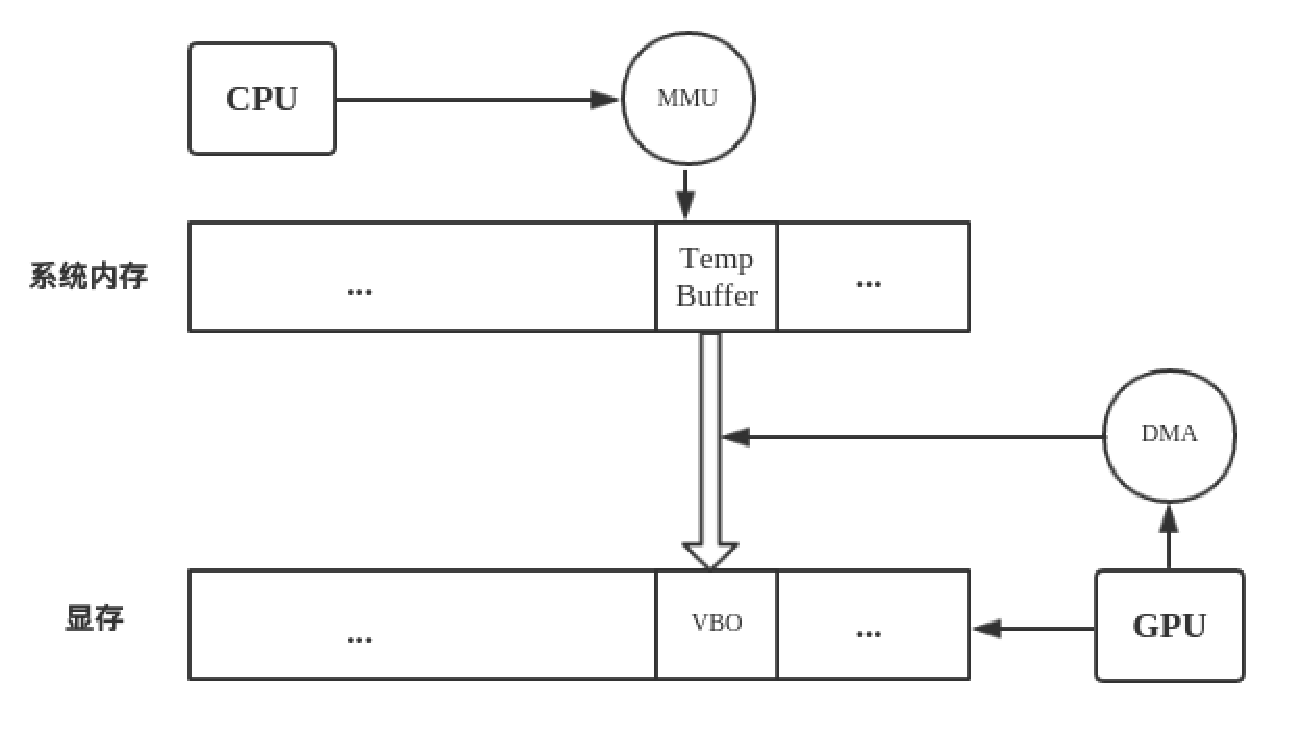
\includegraphics[width=12cm,height=8cm]{figures/chap03/gpu-dma}
  \caption{DMA方式下的Mesa3D库CPU与GPU访存策略}
  \label{fig:gpu-dma}
\end{figure}

改进的传输模式如图\ref{fig:gpu-dma},对比之前的实现(图\ref{fig:vbo-gtt}),虽然设计上更加复杂了一些,但是在龙芯平台上,PCI-E总线带宽较小,直接读写的速度非常慢, 这会导致即使在小数据量时直接读写的效率也比DMA方式的效率更低。


\section{Mesa3D的CPU端计算优化}

\subsection{研究背景}

\subsubsection{CPU的流水线结构和指令级并行}

无论现代CPU的设计如何的复杂,CPU指令的执行都是分步骤按照流水线一样一级一级执行的,最简单的CPU流水线结构把一条指令的执行分为5个阶段:取指(IF)、译码(ID)、执行(EX)、访存(MEM)、写回(WB),称为五级流水\cite{huweiwu}。如图\ref{fig:cpu-pipeline},在一个周期内,可以有5条指令分别处于不同的流水级并发的执行。

\begin{figure}[H] 
  \centering
  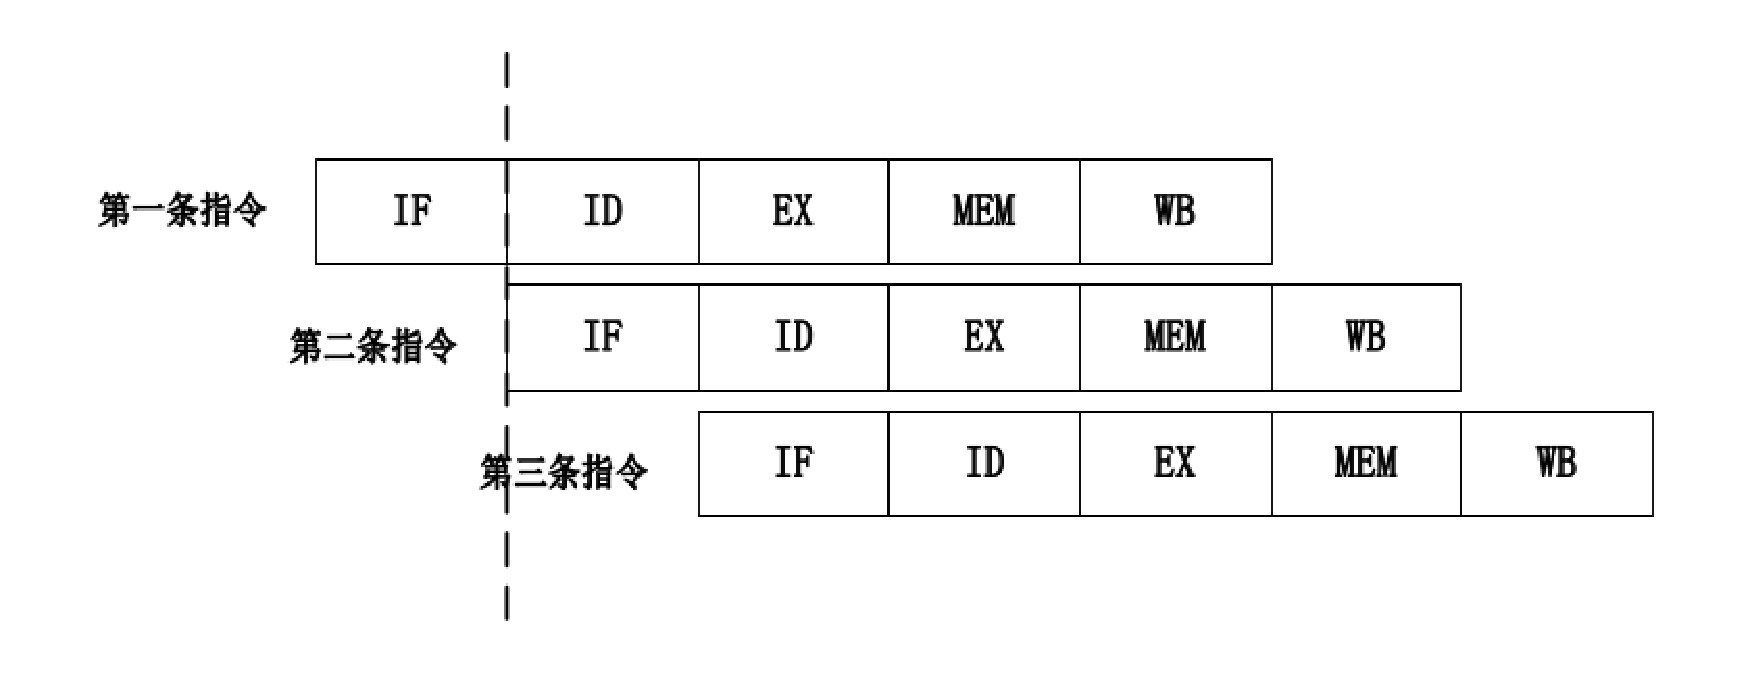
\includegraphics[width=16cm,height=9cm]{figures/chap03/cpu-pipeline}
  \caption{CPU五级流水线结构}
  \label{fig:cpu-pipeline}
\end{figure}

在此基础上,由于硬件设备的增加又产生了多发射的技术,即有多个流水线可以同时执行多条指令。这种指令间的重叠关系称为\textbf{指令级并行}\cite{Quantitative}。影响指令级并行的因素主要有:数据相关、控制相关和结构相关,这里重点介绍以下控制相关:

\textbf{控制相关}:如果两条指令中,有一条指令是转移指令,并且另一条指令是否被执行取决于该转移指令的执行结果,那么它们之间存在控制相关。

为了维护控制相关,现代CPU开发了一套基于硬件的转移推测技术,通过分支历史表(branch history table)来预测分支的转移,如果预测失败则需要重刷流水线,造成性能损失。


\subsubsection{Mesa3D立即模式绘制模式实现原理}


为了说明Mesa3D立即模式的实现原理,这里以svPerfGL的立即模式测试项为例展开分析:

\begin{lstlisting}
	glBegin(GL_TRIANGLES);
	for (i=0; i<tNumVerts; i++){
		glNormal3fv((GLfloat *)(tNorms+i));
		glColor3fv((GLfloat *)(tColors+i));
	    glVertex3fv((GLfloat *)(tVerts+i));
	}
	glEnd();
\end{lstlisting}

这里在一对glBegin和glEnd中间放入了大量的绘制命令,Mesa3D在调用glBegin时候首先会根据绘制图形样式,配置好info.mode信息,例如V\underline{ }008958\underline{ }DI\underline{ }PT\underline{ }POINTLIST、V\underline{ }008958\underline{ }DI\underline{ }PT\underline{ }TRILIST等等。接着会在VRAM上创建一个大小为VBO\underline{ }VERT\underline{ }BUFFER\underline{ }SIZE的空白VRAM空间,这里同样称为buffer0。VBO\underline{ }VERT\underline{ }BUFFER\underline{ }SIZE的默认值为1024*64。接着glBegin与glEnd中间的相关顶点数据就会通过宏函数ATTR(A, N, T, V0, V1, V2, V3)拷贝到buffer0中,当buffer0装满数据后,Mesa3D会备份边界顶点数据,然后将绘制命令发送给GPU进行渲染:

\begin{lstlisting}
r600_write_config_reg(cs, R_008958_VGT_PRIMITIVE_TYPE,
                      r600_conv_pipe_prim(info.mode));
cs->buf[cs->cdw++] = PKT3(PKT3_DRAW_INDEX_AUTO, 1, 
                          rctx->b.predicate_drawing);
cs->buf[cs->cdw++] = info.count;
cs->buf[cs->cdw++] = V_0287F0_DI_SRC_SEL_AUTO_INDEX |
                     (info.count_from_stream_output? 
                         S_0287F0_USE_OPAQUE(1) : 0);
\end{lstlisting}

之后创建新的buffer1来处理后续的顶点数据,如此反复直到glBegin和glEnd里面的数据全都装载完毕并交给GPU处理。简单来说整个过程就是如图\ref{fig:immediate-mode-flow}所示。这里与图\ref{fig:display-list-flow}里面的显示列表实现机制的不同在于显示列表机制下只需要进行一次的数据装载,以后每次调用显示列表时候就不必再数据装载了,而立即模式下每次调用都需要重新的数据装载。

\begin{figure}[H] 
  \centering
  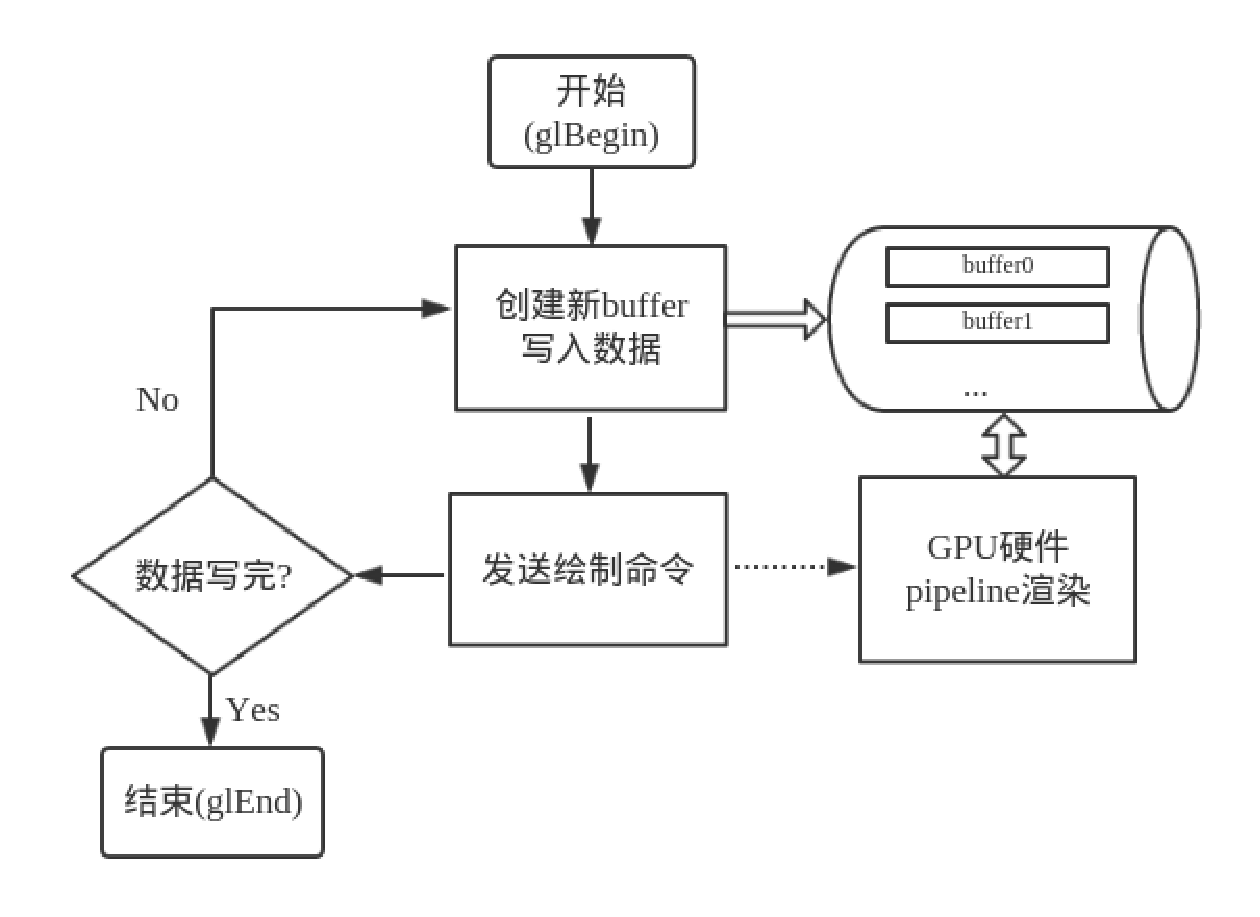
\includegraphics[width=14cm,height=10cm]{figures/chap03/immediate-mode-flow}
  \caption{Mesa3D图形库立即模式实现机制}
  \label{fig:immediate-mode-flow}
\end{figure}

\subsection{CPU端计算热点分析}

我们通过perf性能分析工具分析svPerfGL程序立即模式测试项,测试每帧绘制100万个三角形,绘制60秒后得到相关总体性能参数如下:

\begin{center} \tablecaption{svPerfGL立即模式测试项总体性能分析 \label{tab:imm-perf-stat}} 
\tablefirsthead{
\rowcolor[gray]{0.8}
\multicolumn{1}{c}{\textbf{性能参数项}} &
\multicolumn{1}{c}{\textbf{数值}} \\ }
\tablehead{\multicolumn{2}{c}{
\small 表 \ref{tab:imm-perf-stat} (续) } \\
\rowcolor[gray]{0.8}
\multicolumn{1}{c}{\textbf{性能参数项}} &
\multicolumn{1}{c}{\textbf{数值}} \\ }
\tabletail{\bottomrule
\multicolumn{2}{c}{\small 接下页} \\}
\tablelasttail{\bottomrule}

%./svPerfGL -i ../../trisNormsColors-512.nc -w 1280 -h 1024 -2 -v -t 60 -s 3000000
\begin{supertabular}{p{6.cm}p{6.cm}}
	task-clock& 114772\\
	context-switches& 1104\\
	CPU-migrations& 29\\
	page-faults& 21416\\
	cycles & 102945713309\\
	instructions& 56907962593\\
	branches& 8563703440\\
	branch-missess& 836558158\\
\end{supertabular}
\end{center}

此外,使用perf分析测试程序的热点代码后,得到占总程序一半左右的执行时间比例的热点代码段是前面章节分析提到的宏函数ATTR(具体代码参考附录\ref{cha:attr})。



% 分支预测失败率统计

\subsection{CPU端优化技术}

针对前一节的性能分析结果,本节围绕ATTR宏函数的代码特点提出了两种优化方法:

\begin{itemize}

\item{\textbf{分支结构优化}}

从性能分析表\ref{tab:imm-perf-stat}可以看出,总体的分支预测失败率较高(9.77$\%$)。具体到Mesa3D图形库热点代码ATTR宏函数\ref{cha:attr}实现来看就是以下几行代码造成的:

\begin{lstlisting}
if (N>0) dest[0] = V0;						\
if (N>1) dest[1] = V1;						\
if (N>2) dest[2] = V2;						\
if (N>3) dest[3] = V3;						\
\end{lstlisting}

因为ATTR宏函数是glVertex、glColor和glTexCoord等函数的具体实现函数,就以glVertex浮点类型为例,根据参数个数的不同OpenGL接口就定义了glVertex1f、glVertex2f、glVertex3f和glVertex4f等几种,所以上述代码里面的N就对应glVertex函数的参数个数。那么我们假设在上层应用情景中调用glVertex浮点函数时候glVertex1f、glVertex2f、glVertex3f和glVertex4f的调用频率分别为$f_1, f_2, f_3和f_4$,那么很显然有:
$$
f_1 + f_2 + f_3 + f_4 = 1
$$

由于N为1,2,3和4时候在上述代码段分别需要分支跳转判断都是4次,所以glVertex浮点函数分支跳转在执行上述代码段的平均跳转期望次数就是:

$$f_1*4 + f_2*4 + f_3*4 + f_4*4 = 4$$

这里很显然可以发现上述代码中很多判断是重叠的,比如N是否大于1这个判断是N是否大于2这个判断的真子集,即N大于2成立便可推导出N大于1,不必再进行判断。所以基于这个发现,本文改进了这个判断过程,改进后结果如下:

\begin{lstlisting}
switch(N){	\
case 4: dest[3] = V3;						\
case 3: dest[2] = V2;						\
case 2: dest[1] = V1;						\
case 1: dest[0] = V0;						\
default: \
} \
\end{lstlisting}

改进后代码跳转期望次数为:

$$f_1 * 4 + f_2 * 3 + f_3 * 2 + f_4 * 1 < 4$$

所以从根本上减少了分支跳转代码,缓解了因龙芯平台分支预测率较低带来的性能损失。

\item{\textbf{循环优化}}

除了上面分析的分支跳转的CPU端性能瓶颈以外,还存在着一些循环相关的性能瓶颈。针对这一类的瓶颈主要采用循环展开和循环化简的优化方法。

例如热点循环:
\begin{lstlisting}
for i \leftarrow 1 to n {
	memcpy(A, B, m*sizeof(typeof(A)))
	A \leftarrow A + m;
	B \leftarrow B + m;
}
}
\end{lstlisting}
这个循环就可以直接进行进行循环化简,变成memcpy(A, B, n*m*sizeof(A)),这样做的好处在于减少了glibc库函数memcpy的调用次数,优化之前需要调用n次,优化后只需要调用一次,减少了函数调用的开销。

其他的例如一些宏函数,由于编译器的保守原因,对宏函数里面的循环展开不够,例如ATTR里面的for循环就可以采用循环展开优化性能。

\item{\textbf{MIPS64编译优化}} \\
由于龙芯平台的历史发展原因,很多MIPS32\cite{Mips}的指令的硬件支持不够,譬如sqrt指令都是通过大量的运算指令软件模拟实现的,而后来随着硬件的发展和编译器的优化,龙芯发展出了MIPS64指令集,该指令集硬件支持更好,编译器编译出的汇编指令执行效率更高,所以龙芯3A平台Mesa3D库采用MIPS64编译优化以提高CPU端的计算性能。


\end{itemize}


\section{本章小结}
本章分三个部分分别阐述龙芯平台Mesa3D图形库的优化方法。首先从CPU与GPU的负载均衡的角度上展开程序分析并提出优化策略,以实现CPU和GPU的负载均衡。接着从CPU与GPU的数据传输角度来分析Mesa3D的性能瓶颈,仔细分析了现有Mesa3D内存到显存的传输策略后,采用一种改进的传输优化策略。最后介绍了CPU端计算热点的一些优化手段。
